\section{Условие}
{\bfseries Цель работы:} Научиться конфигурировать многоуровневые коммутаторы $L2/L3$ с $VLAN$, $RSTP$, $LACP$, использовать $inter-VLAN\;routing$, 
настраивать статическую маршрутизацию и конечный пользовательский $NAT$ на $Cisco$.

{\bfseries Вариант:} 29.

\begin{figure}[h!]
    \centering
    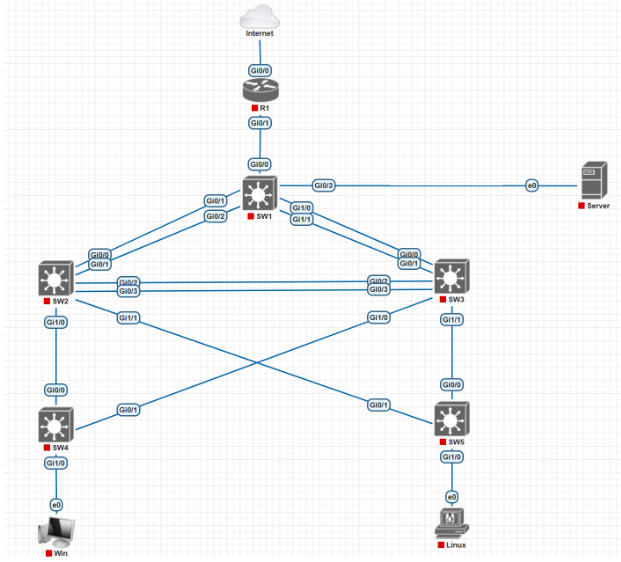
\includegraphics[scale=0.75]{./img/sheme.png}
    \caption{Схема сети}
\end{figure}

{\bfseries Задачи:}
\begin{enumerate}
    \item Настроить имена узлов для коммутаторов и маршрутизатора в соответствии с именами, указанными в топологии.
    \item Сменить пароль администратора (пароль доступа к привилегированному режиму $enable$ для $Cisco$) на вариант ЛР для соответствующего устройства.
    \item Создать пользователя $checker$ с максимальным административным уровнем доступа и паролем “PfxtvXtrth!” без кавычек на коммутаторе и маршрутизаторе.
    \item Настроить на маршрутизаторе $R1$ IP-адреса интерфейсов в соответствии с вариантом задания.
    \item Настроить на маршрутизаторе $R1$ встроенный DNS-сервер с передачей запросов на сервер $QuadNine$ (9.9.9.9), включить удаленные запросы.
    \item Переключить интерфейсы коммутаторов опорной сети в режим $trunk$ $802.1q$ за исключением access-портов ($GigabitEthernet1/0$) на $SW4$ и $SW5$.
    \item Организовать на коммутаторах $SW1$, $SW2$, $SW3$ группы портов между соседними коммутаторами в кольце в каналы $EtherChannel$ в режиме $LACP active$, перевести каналы $EtherChannel$ в транк $802.1q$.
    \item Настроить $VLANs$ на коммутаторах в соответствии с таблицей конфигурации в варианте вручную или (*) с помощью $VTP$.
    \item Настроить $STP$ на коммутаторах таким образом, чтобы для всех $VLAN$ $SW1$ являлся $root\;bridge$, а на коммутаторах $SW4$ и $SW5$ root-портами являлись интерфейсы $GigabitEthernet0/0$.
    \item Разрешить на всех транковых портах коммутаторов только $VLAN$ из таблицы в явном виде. На интерфейсе $GigabitEthernet0/0$ на коммутаторе $SW1$ (в сторону маршрутизатора $R1$) разрешить только $VLAN\;Internet$.
    \item Настроить на коммутаторе $SW1$ IP-адрес на интерфейсе $VLAN\;Internet$ в соответствии с вариантом задания, адрес DNS-сервера (адрес маршрутизатора $R1$) и маршрут по умолчанию на маршрутизатор $R1$.
    \item На коммутаторе $SW1$ назначить IP-адреса во всех $VLAN$ и включить $ip\;routing$.
    \item Назначить IP-адреса в $Management\;VLAN$ на всех коммутаторах согласно варианту и установить маршрут по умолчанию на адрес коммутатора $SW1$.
    \item Настроить на всех коммутаторах в качестве DNS-сервера адрес маршрутизатора $R1$.
    \item Настроить на маршрутизаторе $R1$ статические маршруты на сети из таблицы $VLAN$, ведущие на коммутатор ядра $SW1$.
    \item Настроить на маршрутизаторе $R1$ трансляцию адресов ($NAT$) для доступа в интернет IP-адресов из $VLAN\;Internet$, используя в качестве глобального адреса адрес на интерфейсе $GigabitEthernet0/0$.
    \item Настроить на коммутаторе $SW1$ DHCP-сервер во $VLAN\;Internet$ и $Cash$, используя пулы адресов с маской /24, маршрут по умолчанию на $SW1$ и DNS-сервер на $R1$. Назначить исключения в пулах для статических адресов, назначенных сетевым устройствам.
    \item Перевести порты $GigabitEthernet1/0$ на коммутаторах $SW4$ и $SW5$ в режим $access$ и назначить им $VLAN\;Internet$ ($SW4$) и $Cash$ ($SW5$) соответственно. Проверить доступ в Интернет с узла $Win$ ($Windows 10$) в режиме $DHCP$.
    \item Настроить сервер $Server$ под управлением $Ubuntu\;20.04$ интерфейс $eth0$ в режиме $trunk\;802.1Q$ со всеми $VLAN$ из таблицы, используя $netplan$ и статические адреса из варианта. Проверить доступ в Интернет с сервера, а также доступ к серверу с узла $Win$ и узла $Linux$.
\end{enumerate}

{\bfseries Допустимые средства конфигурации:} Разрешается использовать консоль маршрутизатора и коммутаторов без ограничений. Запрещается использовать web-интерфейс для настройки коммутаторов и маршрутизатора.

\pagebreak